\documentclass[10pt]{article}

%AMS-TeX packages
\usepackage{amssymb,amsmath,amsthm} 
%geometry (sets margin) and other useful packages
\usepackage[margin=1.25in]{geometry}
\usepackage{graphicx,ctable,booktabs}
\usepackage{verbatim}
\usepackage{color}
\usepackage{listings}
\lstset{ %
language=C,                % choose the language of the code
basicstyle=\footnotesize,       % the size of the fonts that are used for the code
numbers=left,                   % where to put the line-numbers
numberstyle=\footnotesize,      % the size of the fonts that are used for the line-numbers
stepnumber=1,                   % the step between two line-numbers. If it is 1 each line will be numbered
numbersep=5pt,                  % how far the line-numbers are from the code
backgroundcolor=\color{white},  % choose the background color. You must add \usepackage{color}
showspaces=false,               % show spaces adding particular underscores
showstringspaces=false,         % underline spaces within strings
showtabs=false,                 % show tabs within strings adding particular underscores
frame=single,           % adds a frame around the code
tabsize=2,          % sets default tabsize to 2 spaces
captionpos=b,           % sets the caption-position to bottom
breaklines=true,        % sets automatic line breaking
breakatwhitespace=false,    % sets if automatic breaks should only happen at whitespace
escapeinside={\%*}{*)}          % if you want to add a comment within your code
}

%
%Fancy-header package to modify header/page numbering 
%
\usepackage{fancyhdr}
\pagestyle{fancy}
%\addtolength{\headwidth}{\marginparsep} %these change header-rule width
%\addtolength{\headwidth}{\marginparwidth}
\lhead{CS 261 Project Report}
\chead{} 
\rhead{\thepage} 
\lfoot{\small Andrew Johnson and Scott Moore} 
\cfoot{} 
\rfoot{\footnotesize CS 261 Project Report} 
\renewcommand{\headrulewidth}{.3pt} 
\renewcommand{\footrulewidth}{.3pt}
\setlength\voffset{-0.25in}
\setlength\textheight{648pt}

\usepackage[square,numbers]{natbib}

%%%%%%%%%%%%%%%%%%%%%%%%%%%%%%%%%%%%%%%%%%%%%%%

\usepackage{trfrac}
\newcommand{\sign}[2]{\ensuremath{#1\;\textsf{signed}\;#2}}
\newcommand{\imp}[2]{\ensuremath{#1 \rightarrow #2}}
\newcommand{\says}[2]{\ensuremath{#1\;\textsf{says}\;#2}}
\newcommand{\confirms}[2]{\ensuremath{#1\;\textsf{confirms}\;#2}}
\newcommand{\ctxt}[0]{\ensuremath{\Gamma}}
\newcommand{\nil}[0]{\ensuremath{\cdot}}
\newcommand{\bnfsep}[0]{\ensuremath{\;\mid\;}}
\newcommand{\entails}[2]{\ensuremath{#1 \vdash #2}}
\newcommand{\pred}[2]{\ensuremath{\textsc{#1}(#2)}}
\newcommand{\subst}[2]{\ensuremath{[#1/#2]}}
\newcommand{\abs}[1]{\ensuremath{\forall x:\;#1}}
\newcommand{\rtcheck}[0]{\ensuremath{\textsf{Runtime check}}}
\newcommand{\with}[1]{\ensuremath{\;(\text{with } #1)}}
\newcommand{\todo}[1]{{\color{red}todo: {#1}}}

\begin{document}

\title{Authorization Logic in JOS}
\author{Andrew Johnson and Scott Moore}

\maketitle

\thispagestyle{empty}

\begin{section}{Introduction}
Authorization logics are a principled technique for implementing rule-based access control mechanisms.
They have several advantages over traditional OS access control mechanisms such as access control lists.
In particular, they allow principals to express access control decisions for which they do not have complete information.
Authorization logics also provide \emph{proof-carrying authorization}. That is, the capability to access a resource carries with it the set of authorization decisions that granted it.
\todo{more introduction}

\subsection{Related work}
\todo{more information and reword some}
There has been quite a lot of work on authorization logics, particularly in the context of distributed systems.
Most recently, \citet{Nexus} developed the Nexus operating system, which uses authorization logic to combine different trust bases for secure systems into a cohesive authorization system.
Our system borrows Nexus's authority mechanism to allow revocation and other dynamic authorization policies.

Our authorization logic is based on \citet{Bauer}'s authorization logic extended with a primitive for dynamic authorization checks and cut elimination, which reduces the size of proofs.
More sophisticated authorization logics are given by \citet{AURA} and \citet{Garg}.

\todo{relationship to capabilities}
\end{section}

\begin{section}{Design}

We replaced the current authorization mechanism for JOS system calls (\textsf{envid2env}) with a new mechanism based on authorization logic. Principals (environments) use a secure binding to specify an authorization goal which is used to mediate access to system calls affecting the environment.
An authorization goal is a formula in our authorization logic. Access is granted to any principal presenting a proof of the authorization goal.

Formulas in our logic have the following syntax: \\[1em]
\begin{tabular}{llcl}
\emph{principals} & R & ::= & $x$ \bnfsep $v$ \\
\emph{predicates} & P & ::= & $pred(R)$ \\
\emph{formulas} & F & ::= & $P$ \bnfsep \imp{F_1}{F_2} \bnfsep \abs{F} \bnfsep \sign{A}{F} \bnfsep \says{A}{F} \bnfsep \confirms{A}{F}\\
\emph{contexts} & \ctxt & ::= & \nil \bnfsep \ctxt,$F$ \\
\end{tabular} \\[1em]

Formulas include first order predicates over principals, implication, and universal quanitification over principals. Conjunction can be encoded as implication ($A \wedge B \implies C \equiv A \implies B \implies C$). The remaining formulas describe a principal's beliefs. The formula \says{A}{F} can be interpreted as ``principal $A$ believes the formula $F$ to be true.'' In general, we can infer statements of this form by logical inference from the set of initial beliefs of the principal and the beliefs of other principals. We distinguish between two types of belief: these initial, or \emph{asserted}, beliefs and derived beliefs.

The inference rules for our logic are given in Figure~\ref{fig:logic}.
Our logic is also constructive, and thus proofs not only demonstrate a capability to access a resource, but an audit trail describing how that access was granted.

\begin{figure}
\center
$\trfrac[\;signed]{\rtcheck}{\entails{\ctxt}{\sign{A}{F}}}$ \hfil
$\trfrac[\;confirms]{\rtcheck}{\entails{\ctxt}{\confirms{A}{F}}}$ \hfil
$\trfrac[\;assump]{F \in \ctxt}{\entails{\ctxt}{F}}$ \\[1em]

$\trfrac[\;tauto]{\entails{\ctxt}{F}}{\entails{\ctxt}{\says{A}{F}}}$ \hfil
$\trfrac[\;weaken impl]{\entails{\ctxt,F_1}{F_2}}{\entails{\ctxt}{\imp{F_1}{F_2}}}$ \hfil
$\trfrac[\;impl]{\entails{\ctxt}{F_1} \quad \entails{\ctxt}{\imp{F_1}{F_2}}}{\entails{\ctxt}{F_2}}$ \\[1em]

$\trfrac[\;sign]{\entails{\ctxt}{\sign{A}{F_1}} \quad \entails{\ctxt,F_1}{\says{A}{F_2}}}{\entails{\ctxt}{\says{A}{F_2}}}$ \hfil
$\trfrac[\;conf]{\entails{\ctxt}{\confirms{A}{F_1}} \quad \entails{\ctxt,F_1}{\says{A}{F_2}}}{\entails{\ctxt}{\says{A}{F_2}}}$ \\[1em]

$\trfrac[\;says]{\entails{\ctxt}{\says{A}{F_1}} \quad \entails{\ctxt,F_1}{\says{A}{F_2}}}{\entails{\ctxt}{\says{A}{F_2}}}$ \hfil
$\trfrac[\;spec]{\entails{\ctxt}{\says{A}{(\abs{F_1})}} \quad \exists p:\;\entails{\ctxt,F_1\subst{p}{x}}{\says{A}{F_2}}}{\entails{\ctxt}{\says{A}{F_2}}}$
\caption{Inference rules of our authorization logic}
\label{fig:logic}
\end{figure}

The meta variable $A$ in the formulas \textsf{signed}, \textsf{says} and \textsf{confirms} ranges over principals.
$P$ would denotes uninterpreted first-order predicates (e.g., \pred{Trusted}{Env}, \pred{Parent}{Env}).
The formula \imp{F_1}{F_2} denotes implication. 

\sign{A}{F} indicates that $A$ believes $F$ to be true; at run time, it corresponds to a digitally signed assertion.
\says{A}{F} denotes that $F$ is a statement which $A$ believes given the formulae asserted by A and the beliefs of other principals.

\paragraph{Example} Suppose that principal $A$ wishes to delegate its authorization decisions to $B$. Then $A$ would assert \sign{A}{\imp{(\says{B}{\pred{OK}{Env}})}{\pred{OK}{Env}}}. Now for any principal $C$ authorized by $B$ (\says{B}{\pred{OK}{C}}), we can derive \says{A}{\pred{OK}{C}}.

\medskip

\confirms{A}{F} is a new formula we are adding to the logic and corresponds with the authority abstraction in the Nexus system \cite{Nexus}. 
\confirms{A}{F} is a \emph{secure binding} of a run time authorization decision to a principal. \confirms{A}{F} is validated by invoking a decision procedure in $A$ that takes the authorization formula $F$ as input and returns true if $A$ believes $F$.
Crucially, checking the validity $\confirms{A}{F}$ does not create a reusable proof object.
This allows time-sensitive or revocable authorization decisions to be implemented on top of our simple logic without explicitly incorporating time or revocation as primitives.
\end{section}

\begin{section}{Implementation}

We broke implementation into three stages.  We first embedded our logic into the Coq Proof Assistant.  Second, we ported that code to C as a stand-alone library.  Third, we integrated the library into the JOS operating system.
\subsection{Coq}
In order to ensure the correctness and completeness of our logic and proof checker, we first embedded it into the Coq Proof Assistant.  This enabled us to prove that our proof checker was correct and always terminated, as well as work out some of the implementation details in a strongly typed language.  For example, we first defined variables as strings and carried an environment mapping names to values.  This made the proof checker overly complicated and stripping it out led to a far simpler implementation both in Coq and C.  Writing the proof checker in Coq allowed us to prove that it was correct (in fact, using Coq's dependent types, we actually return the Coq proof that the proof checker is correct from the check function).  We therefore can be assured that we did not skip any corner cases, or over-simplify.  The logic, proof checker, and examples were implemented in about 400 lines in Coq.
\subsection{C Library} \label{sec:clib}
There is no way to directly compile Coq code into C code, so we performed this translation by hand.  This obviously invalidates our proof of correctness.  By using Coq, we gained the fact that our algorithms and data structures were correct, but have no such guarantee for the C implementation.  We compensated for this by writing a number of tests (now in \textsf{user/proof\_test.c}).  The C library implements the logic and inference rules as in Figure \ref{fig:logic}.  For ease of use we also implemented constructors for primitive proofs, primitive formulas, principals, and for more complex, commonly used, proofs.  The Context, shown as $\Gamma$ in Figure \ref{fig:logic}, was implemented as a stack of formulas since the proof checker adds a formula to the context and, once it has been used, removes that formula.  Formulas and Proofs are represented as tagged \textsf{union}s of the primitive types together with an \textsf{enum} indicating the current type (another option would be to use C++ subclassing).  
\newline\newline
To simplify memory management, all constructors perform a deep copy of all input data structures.  This means that a proof can be freed without worrying about the constituent subproofs and formulas.  To make this approach easy to implement, each of the data structures has a comparison function and a deep-copy function.  In addition, to ease debugging and introspection, each data structure can be printed (recursively) as a pre-formatted \LaTeX{ }string (many examples of which are in this document).  In total, the library implementation consists of approximately 2600 lines of C, about half of which is test code.

\subsection{JOS Integration}
\begin{figure}
\[
\trfrac[\;sign]{\trfrac[\;signed]{\rtcheck}{\sign{B}{\pred{OK}{A}}} \quad \trfrac[\;tauto]{\trfrac[\;init]{\rtcheck}{\pred{OK}{A}}}{\says{B}{\pred{OK}{A}}}}{\says{B}{\pred{OK}{A}}}
\]
\caption{Simple Attestation Proof}
\label{fig:attest}
\end{figure}
The library described in section \ref{sec:clib} provides a logic and a method to create and check proofs defined in that logic.  In order to use this for authorization we needed to integrate it into an operating system.  We chose to use JOS for simplicity; the existing authorization mechanism was easy to replace.  We chose to focus on replacing environment to environment authentication.  In JOS, an environment is authorized to manipulate another only if it is the direct parent environment. We replace this with a more flexible model built on our authorization logic.  Essentially, to manipulate environment $A$, environment $B$ must provide a proof of a logical formula defined by $A$.  These proofs are checked by the JOS kernel. The modular design of our C library allowed us to more or less drop it into JOS as a library.  In order to facilitate this we essentially only needed to implement a JOS memory manager (\textsf{malloc} and \textsf{free}) to replace the \textsf{stdlib} version.
\subsubsection{Environments}
Each environment has the option to define a single logical formula and add a pointer to it to their environment structure.  If environment A defines a formula $F = \pred{OK}{x}$ and sets it with our new $\textsf{sys\_set\_goal}(F)$ system call. Then 
\[
F_{says} = \says{A}{\pred{OK}{x}}
\]
and $F_{says}(x)$ must be proved for environment $x$ to manipulate $A$.  If environment $B$ has a proof, $P$, of $F_{says}(B)$ then $B$ adds a pointer to this proof in their environment structure with $\textsf{sys\_set\_proof}(P)$ before making a system call that would affect environment $A$.
\subsubsection{System Calls}
If a system call, say \textsf{sys\_page\_map}, will affect a environment $A$ then, when $B$ makes that call, the JOS kernel uses the proof, $P$, that $B$ put into their environment structure and checks that $P$ is a valid proof of the formula, $\says{A}{F(B)}$, where $F$ is what $A$ has indicated.  Setting $F$ in $A$ and setting $P$ in $B$ are both accomplished using system calls.  We also add a system call, \textsf{sys\_sign\_formula}, for signing formulas, rather than implementing cryptographic digital signatures.  The kernel stores a list of all signed formulas and checks this list when checking a proof.  See Listing \ref{code:attest} for a simple example; setting up a proof goal and constructing and using the proof in Figure \ref{fig:attest}.
\lstset{language=C,caption={Environment $A$ constructs a proof goal, $F$, and signs $F(B)$.  Environment $B$ creates and uses a proof of $\says{A}{F(B)}$ depending on the fact that $A$ signed $F(B)$.},label=code:attest}
\begin{lstlisting}
// Constructed in A

// This is equivalent to [for all x, OK(x)]
// What will actually be proved is [A says OK(B)] where B has been substituted for x
Formula F = formula_pred(OK, x);
sys_set_goal(F);
sys_sign_formula(formula_subst(F, x, B));

// Constructed in B

// Proof of [A says F(B)]
Formula F_B_subst = formula_pred(OK, B);
Proof P  = says_from_signed(A, F_B_subst);
sys_set_proof(P);
...
// Map a page from B to A
sys_page_map(0, Bvaddr, A, Avaddr, perm);
\end{lstlisting}
\subsubsection{Runtime Verification}
During proof checking there are three runtime checks, context membership, signatures, confirmations.  The first is straightforward list inclusion, and the second is implemented as a special case of the first.  The third, confirmation, relies on code that is defined by the confirming environment.  By making the system call, \textsf{sys\_set\_confirms\_upcall}, the confirming environment, $A$, can set a function that should be called to check any statement of the form $\confirms{A}{F}$.  At runtime a candidate Formula is passed into the upcall, which returns a boolean value.  In our implementation we run this code in the proof checker (in the kernel), assuming it is well behaved (terminates, does not abuse privilege).  A future implementation could restrict upcalls to well-behaved functions and check this property at runtime.  
\subsubsection{Proof Sharing}
It can be easier to construct a proof or parts of a proof in the environment which defines the goal to be proved.  In these cases the proofs need to be handed out to the provers.  To do this we created library functions to send and receive proofs.  These are implemented on top of IPC, adding handling of dynamically allocated data structures.  We can achieve the same result as in Listing \ref{code:attest} using proof sharing as seen in Listing \ref{code:share}.
\lstset{language=C,caption={Environment $A$ constructs a proof and sends it to environment $B$, which then uses the proof.},label=code:share}
\begin{lstlisting}
// Constructed in A
Formula F = formula_pred(OK, x);
sys_set_goal(F);
// This automatically calls sys_sign_formula when called from A
Proof P  = says_from_signed(A, formula_subst(F, x, B));
send_proof(B, P);

// Constructed in B
Proof P = receive_proof();
sys_set_proof(P);
...
// Map a page from B to A
sys_page_map(0, Bvaddr, A, Avaddr, perm);
\end{lstlisting}

\subsubsection{Proof Caching}\label{sec:cache}
We implement a simple form of proof caching.  If the proof checker returns true, we add that proof's goal to a persistent context located in the kernel.  When a proof is checked we first check whether the proof's goal is already in the kernel's context.  If it is then we immediately return true.  Note that we should not cache any proofs using confirmation, since this is a dynamic runtime check.  In our proof of concept proof-caching we do not take this into account.  The effects of caching can be seen in the Section \ref{sec:eval}.

\subsubsection{User Programs}
\paragraph{prooftest} Contains tests for functions pertaining to building, printing, and copying Formulas and building, printing, copying, and checking Proofs.
\paragraph{prooftimertest} Implements infrastructure used for performance testing.
\paragraph{authtest} Builds and uses simple attestation proof as in Listing \ref{code:share}.
\paragraph{confirmstest} Sets a confirms up call and creates a proof that uses it.
\paragraph{fratricide} The parent environment forks 10 children.  Each one delegates to the parent.  The parent then spawns the 11th child, call him Killer, and signs a statement that Killer is OK.  The parent then exits gracefully, and Killer senselessly \textsf{sys\_env\_destroy}s the other 10 children before \textsf{sys\_env\_destroy}ing himself.
\paragraph{authmemmap} The parent environment forks 2 children.  Each delegates to the parent who then signs that the second environment is OK.  The second environment is then able to map a number of pages into the first environment with a single IPC message, which is used only for synchronization.  Previously each page would need to be shared via a separate IPC message.  (Note that occasionally this program runs into a race condition where the IPC message was received, but the receiving environment still page faults.  This appears to be unrelated to our authorization logic additions.)
\paragraph{authcompare} This program sets up the logic to compare mapping memory using runtime authorization and \textsf{sys\_page\_map} to using IPC.  The goal is to map 1000 pages from one environment to another.  The authorization logic setup is the same as in \textsf{authmemmap}.  When using IPC, the sender loops, calling \textsf{ipc\_send} and the receiver loops, calling \textsf{ipc\_receive}.
\end{section}

\begin{section}{Evaluation}\label{sec:eval}
\subsection{Performance}
\begin{figure}
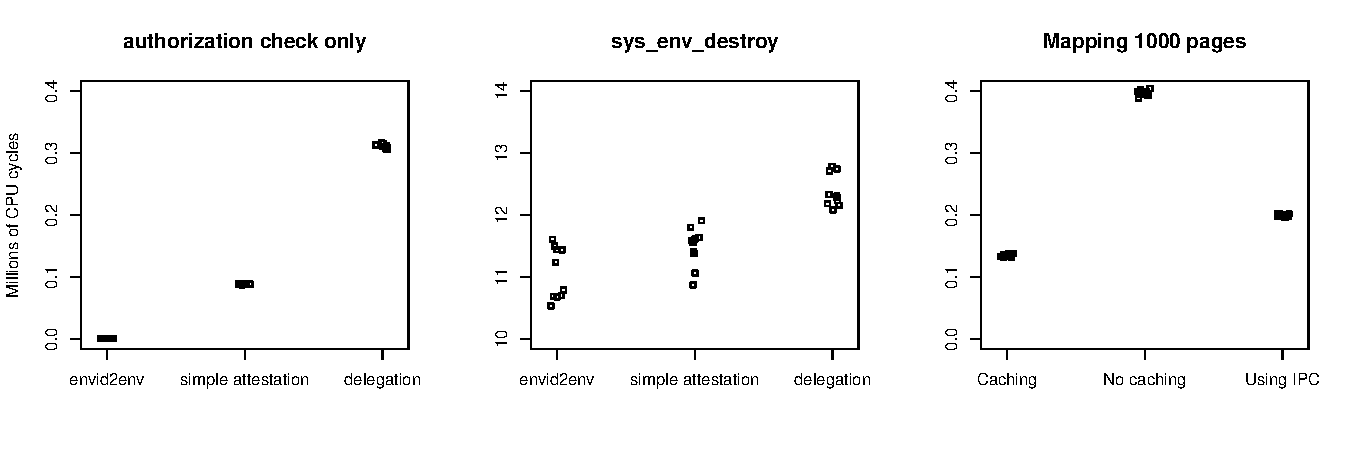
\includegraphics[width=\textwidth]{plots.pdf}
\caption{The left and center plots show the performance of authorization logic proof checking compared with previous JOS mechanism.  The right plot shows the effect of proof-caching and compares mapping 1,000 pages with our authorization checks to sending pages over IPC.}
\label{fig:perf}
\end{figure}
To evaluate the performance of the proof checker in the kernel we implemented a dummy system call that checks authorization and immediately returns.  This also allows for easily checking a proof which turned out to be useful for debugging proof construction.  As seen in Figure \ref{fig:perf}, we compared the performance of the existing parent/child check to that of checking a simple attestation proof as in the example in Listing \ref{code:attest}, and against a more complex delegation proof as described in Section \ref{sec:delegation}.  We measured CPU cycles from within QEMU using rdtsc().  These were measured from the time the system call function was called in the kernel to the time it returns so it does not include any kernel crossings.  The left and center plots in Figure \ref{fig:perf} use no proof-caching, so this is roughly equivalent to checking a different proof in each system call.  The left plot in Figure \ref{fig:perf} shows the number of cycles for just the authentication checks.  Each circle is the average of 40,000 calls for \textsf{envid2env} and attestation and 1500 calls for delegation.  The center shows the number of cycles for the \textsf{sys\_env\_destroy} function call.  Each circle in this plot is a single call to \textsf{sys\_env\_destroy}. (Note that we made many other system calls prior to \textsf{sys\_env\_destroy} since the first system call took significantly longer in each case due to what we assume were cache effects).
\newline\newline
The left plot in Figure \ref{fig:perf} shows a significant amount of slowdown.  The simple attestation is about 110 times slower than the simple parent/child check, and checking delegation is approximately 3.5 times slower than the simple check.  The proof for attestation can be seen in Figure \ref{fig:attest} and the proof for delegation in Figure \ref{fig:delegation}.  Each horizontal line is effectively either a runtime check or a run of the proof checker.  The simple proof has 4 checks while the delegation proof has 12, so, as expected, we see an approximately linear slowdown with increased proof complexity.  In the center of Figure \ref{fig:perf} we see that the work done by a complex system call, such as \textsf{sys\_env\_destroy}, dominates the proof checking time with less than 5\% slow down for simple proof checking and less than 15\% slowdown for the delegation proof.  Note that the delegation proof is enabling environment interactions that would be impossible in the parent/child scheme, an environment can fall back on the fast parent/ child check by setting their goal to \textsf{NULL}.  Any scheme performing more complex checks would inevitably be slower, but we probably see additional slowdown as we trade performance for flexibility and generality.  In addition we end up doing a lot of unnecessary memory copying to simplify memory management.
\subsubsection{Proof Caching}\label{sec:cacheperf}
Some of this performance can be gained back without sacrificing functionality.  Something that was successful in Nexus was proof-caching \cite{Nexus}.  For frequently used proofs we could cache the proof checker output in the kernel, or at least cache the parts that do not require dynamic runtime checks (everything but confirmation verifications).  Not in Nexus, environments could also provide a proof-caching service.  An environment, $A$, would be presented with a valid complex proof of $\says{A}{F}$ and sign a copy of $F$, which can then be used in place of the original proof.  We leave this as future work.
\newline\newline
As discussed in Section \ref{sec:cache} we implemented a rudimentary proof-caching mechanism within the kernel. The center plot of Figure \ref{fig:perf} shows the effects of proof caching.  As expected we see a dramatic reduction in authorization time.  In fact, with proof-caching, we can map 1,000 pages faster than we can send them over IPC.  Without proof-caching, authorization checks take about twice the amount of time as sending IPC messages.
\subsection{Usability}
\todo{pretty print}
\newline
\todo{helper constructors}

\end{section}
\begin{section}{Example: Delegation}\label{sec:delegation}
Suppose an environment wishes to accept as ``OK'' whatever another environment accepts as ``OK''.  This is a fairly common type of proof called delegation.  Consider the following example.  We have a parent environment, $P$, and two child environments, $C_1$ and $C_2$.
$C_2$ delegates to $P$.  $C_1$ uses this fact along with the fact that $\sign{P}{\pred{OK}{C_1}}$ to prove $\says{C_2}{\pred{OK}{C_1}}$.  This will allow $C_1$ to make system calls affecting $C_2$, such as $\textsf{sys\_page\_map}$.  A typical proof using delegation can be seen in Figure \ref{fig:delegation}.  We have added helper functions to create these proofs.  The use of these to construct a proof can be seen in Listing \ref{code:delegation}.
\newline\newline
\begin{figure}
$
P_1 = \trfrac[\;sign]{\trfrac[\;signed]{\rtcheck}{\sign{C_2}{\abs{\imp{\says{P}{\pred{OK}{v_{0}}}}{\pred{OK}{v_{0}}}}}} \quad \trfrac[\;tauto]{\trfrac[\;assump]{\rtcheck}{\abs{\imp{\says{P}{\pred{OK}{v_{0}}}}{\pred{OK}{v_{0}}}}}}{\says{C_2}{\abs{\imp{\says{P}{\pred{OK}{v_{0}}}}{\pred{OK}{v_{0}}}}}}}{\says{C_2}{\abs{\imp{\says{P}{\pred{OK}{v_{0}}}}{\pred{OK}{v_{0}}}}}} \\\\\\\\
P_2 = \trfrac[\;tauto]{\trfrac[\;impl]{\trfrac[\;sign]{\trfrac[\;signed]{\rtcheck}{\sign{P}{\pred{OK}{C_1}}} \quad \trfrac[\;tauto]{\trfrac[\;assump]{\rtcheck}{\pred{OK}{C_1}}}{\says{P}{\pred{OK}{C_1}}}}{\says{P}{\pred{OK}{C_1}}} \quad \trfrac[\;assump]{\rtcheck}{\imp{\says{P}{\pred{OK}{C_1}}}{\pred{OK}{C_1}}}}{\pred{OK}{C_1}}}{\says{C_2}{\pred{OK}{C_1}}} \\\\\\\\
\text{DELEGATION} = \trfrac[\;spec]{P_1 \quad C_1 \quad P_2}{\says{C_2}{\pred{OK}{C_1}}} \\\\\\\
$
\caption{Delegation Proof}
\label{fig:delegation}
\end{figure}
\lstset{language=C,caption={Delegation using helper functions, proof sharing has been omitted},label=code:delegation}
\begin{lstlisting}
// Constructed in C2
Proof del = delegate_from_signed(C2, P, OK);  

// Constructed in parent
Formula pred = formula_pred(OK, C1);
Proof  perm = says_from_signed(P, pred);

// Constructed in C2
Proof  use_del = use_delegation(C2, P, C1, OK, del, perm);
\end{lstlisting}
In Listing \ref{code:delegation}, $P_1$ is a proof that $C_2$ delegates to $P$ for the OK predicate, and is constructed in line 2 above.  $P_2$ begins with $\sign{P}{\pred{OK}{C_1}}$ and is then used together with $P_1$ to prove $\says{C_2}{\pred{OK}{C_1}}$.  There are runtime checks required by ``signed'' to verify the signatures, and by ``assump'' to verify that the given statement is in the context (note that this proof begins with an empty context, but that the proof checker adds to its context at runtime).  
\end{section}

\begin{section}{Future Work}
\todo{Kernel principal.}\newline
\todo{Multiple goals for a single environment. Multiple up calls}\newline
\todo{Proof caching (also in performance section).}\newline
\todo{Other uses. access control, capabilities}\newline
\end{section}

\begin{section}{Summary}
\end{section}

\begin{section}{Appendix: JOS Changes}
List of files changed in JOS. \newline
\newline
Added:\newline
inc/context.h \newline
inc/env.h \newline
inc/formula.h \newline
inc/mm.h \newline
inc/proof.h \newline
inc/prooflib.h \newline
kern/proofcheck.c \newline
kern/proofcheck.h \newline
lib/context.c \newline
lib/formula.c \newline
lib/mm.c \newline
lib/proof.c \newline
lib/prooflib.c \newline
user/authmapmem.c \newline
user/authtest.c \newline
user/confirmstest.c \newline
user/fratricide.c \newline
user/prooftest.c \newline
user/prooftimertest.c \newline
\newline
Modified: \newline
inc/lib.h \newline
inc/syscall.h \newline
kern/env.c \newline
kern/env.h \newline
kern/syscall.c \newline
kern/trap.c (testing only) \newline
lib/ipc.c \newline
lib/syscall.c \newline
\end{section}

\bibliographystyle{plainnat}
\bibliography{bib}

\end{document}
